\section{Aufbau und Durchführung}
In diesem Versuch wird die Apperatur aus Abbildung \ref{fig:Aufbau} verwendet.
Nachdem überprüft wurde, ob sich die \SI{1}{mm}-Blende und der LiF-Kristall in den jeweiligen Halterungen befinden und ob die Schlitzblende waagerecht zur Drehrichtung ist,
wird das zum Röntgenerät passende Programm gestartet. Im Programm wird daraufhin unter \textit{measure} im Menüpunkt \textit{Messgeräte} das Röntgenerät angewählt.
Für die im folgendem beschriebenden Messungen muss für die Beschleunigungsspannung \SI{35}{kV} und für den Emissionsstrom \SI{1}{mA} gewählt werden.
\begin{figure}[H]
  \centering
  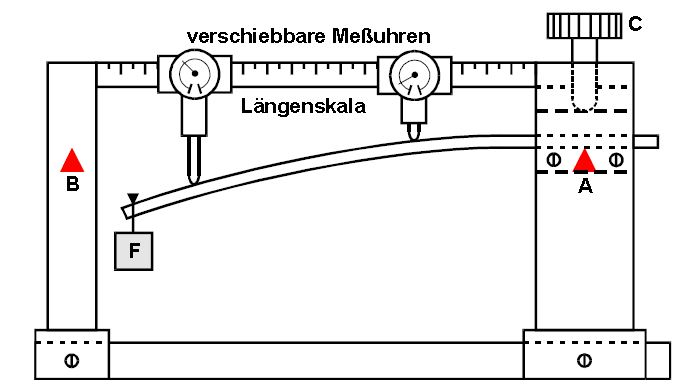
\includegraphics[width=\linewidth-100pt,height=\textheight-100pt,keepaspectratio]{Text/Bilder/Aufbau.png}
  \caption{Röntgengerät \cite[4]{sample}}
  \label{fig:Aufbau}
\end{figure}
In der ersten Messung wird zunächst die Braggbedingung überprüft. Dazu wird der LiF-Kristall auf einen festen Winkel $\phi=14°$ eingestellt.
Daraufhin wird mithilfe des Geiger-Müller Zählrohrs die Röntgen-Intensität im Bereich $26° \le \alpha_\text{GM} \le 30°$  mit einem Winkelzuwachs von $\Delta \alpha = 0,1°$ gemessen.
Für die Integrationszeit wird hier $\Delta t =\SI{20}{s}$ gewählt. \\
In der darauf folgenden Messung wird das Emissionsspektrum einer Cu-Röntgenröhre untersucht. Dazu wird im Programm der $2:1$ Koppelmodus gewählt und im Winkelbereich $4° \le \alpha \le 26°$ die
Röntgenspektrum in $0,2°$-Schritten gemessen. Für die Integrationszeit wird hier $\Delta t = \SI{5}{s}$ gewählt. \\
In der nun beschriebenden Messreihe werden Absorptionsspektren untersucht.
Dazu wird ein Absorber vor das Geiger-Müller Zählrohr gesetzt und das Absorptionsspektrum in $0,1°$-Schritten in einem geeigneten Bereich gemessen. Die Messzeit soll hier
$\Delta t = \SI{20}{s}$ betragen. Dies soll für 4 weitere Materialien mit einer Ordnungzahl von $30 \le Z \le 50$ wiederholt werden. Ebenso soll dies für ein Material mit Ordnungzahl $Z \ge 70$ wiederholt werden.
